F\"ur   die  Regler-Dimensionierung   sowie  das   grafische  Darstellen   der
Schrittantwort  muss   die  Software  einige  Berechnungen   ausf\"uhren.   Im
folgenden  Kapitel werden  die wichtigsten  Schritte dieser  Berechnungen kurz
zusammengefasst und erkl\"art.

\begin{itemize}
    \item
    Bestimmung  des  Frequenzgangs  der  Regelstrecke  aus  Verz\"ogerungszeit
    $T_u$, Anstiegszeit $T_g$ und Verst\"arkung $K_s$.
    \item
    Dimensionierung des Reglers mittels Faustformeln.
    \item
    Dimensionierung des Reglers durch Phasengangmethode.
    \item
    Umrechung der Regler-Darstellung zwischen bodekonformer und reglerkonformer
    Darstlelung. \todo{Erkl\"arung}
    \item
    Berechnung der Schrittantwort des geschlossenen Regelkreises.
\end{itemize}

\subsection{Frequenzgang der Regelstrecke}
\todo{N\"ahere Erl\"auterungen?}
\todo{Bildliche  Illustration   einer  Schrittantwort  der  Strecke   und  des
zugeh\"origen Frequenzgangs?}

F\"ur  die   Identifikation  des   Freqeunzgangs  steht   die  Matlab-Funktion
\code{p2\_sani.m} zur  Verf\"ugung, welche in  der Lage ist, PTn  Strecken mit
einem Grad zwischen 1 und 8 zu identifizieren. Deshalb wird hier nicht n\"aher
auf  die  Berechnung  eingegangen,  da die  Funktion  lediglich  in  Java-Code
``\"ubersetzt'' werden muss.


\subsection{Regler-Dimensionierung mittels Faustformeln}
Im   Praxiseinsatz  stehen   f\"ur   die  Dimensieung   der  Regler   einfache
Berechnungsformeln f\"ur die Einstellwerte der  Regler anhand von $T_u$, $T_g$
und $K_s$ zur Verf\"ugung.

Einige   dieser  Faustformeln   werden  in   der  Applikation   zum  Vergleich
mitberechnet. Die    dazugeh\"origen    Berechnungen    sind    der    Tabelle
\ref{tab:faustformeln} zu entnehmen.

\begin{longtable}{p{50mm}rrrrr}
    \toprule

    %\multicolumn{3}{l}{\large{\textsc{Auftragsanalyse und Hintergrundinformationen}}} \\

    Faustformel
    &
    \multicolumn{2}{l}{PI-Regler}
    &
    \multicolumn{2}{l}{PID-T1-Regler}
    \\

    &
    $T_n$
    &
    $K_p$
    &
    $T_n$
    &
    $T_v$
    &
    $K_p$
    \\

    \midrule

    \endhead
    \endfoot
    \endlastfoot

    % CONTENT HERE ---------------------------------------------------------- %

    \pbox{45mm}{Chiens, Hrones, Reswick \\ \small{\textbf{(0\% \"Uberschwingen)}} \\ \cite{ref:chiens_tsn}, \cite{ref:chiens_wiki}}
    &
    $1.2\cdot T_g$
    &
    $\frac{0.35}{K_s} \cdot \frac{T_g}{T_u}$
    &
    $T_g$
    &
    $0.5\cdot T_u$
    &
    $ \frac{0.6}{K_s} \cdot \frac{T_g}{T_u} $
    \\

    \addlinespace[1em]

    \pbox{45mm}{Chiens, Hrones, Reswick \small{\textbf{(20\% \"Uberschwingen)}} \\ \cite{ref:chiens_tsn}, \cite{ref:chiens_wiki}}
    &
    $T_g$
    &
    $\frac{0.6}{K_s} \cdot \frac{T_g}{T_u}$
    &
    $1.35\cdot T_g$
    &
    $0.47 \cdot T_u$
    &
    $ \frac{0.95}{K_s} \cdot \frac{T_g}{T_u} $
    \\

    \addlinespace[1em]

    Oppelt \cite{ref:op_ros_zieg}
    &
    $3 \cdot T_u$
    &
    $\frac{0.8}{K_s} \cdot \frac{T_g}{T_u}$
    &
    $2 \cdot T_u$
    &
    $ 0.42 \cdot T_u $
    &
    $ \frac{1.2}{K_s} \cdot \frac{T_g}{T_u} $
    \\

    \addlinespace[1em]

    Rosenberg \cite{ref:op_ros_zieg}
    &
    $3.3 \cdot T_u $
    &
    $ \frac{0.91}{K_s} \cdot \frac{T_g}{T_u} $
    &
    $ 2 \cdot T_u $
    &
    $ 0.45 \cdot T_u $
    &
    $ \frac{1.2}{T_s} \cdot \frac{T_g}{T_u}$
    \\

    \addlinespace[1em]

    Ziegler/Nichols \cite{ref:op_ros_zieg}
    &
    $ 3.33 \cdot T_u $
    &
    $ \frac{0.9}{K_s} \cdot \frac{T_g}{T_u} $
    &
    $ 2 \cdot T_u $
    &
    $ 0.5 \cdot T_u $
    &
    $ \frac{1.2}{K_s} \cdot \frac{T_g}{t_u} $
    \\

    \bottomrule
\caption{Faustformeln zur Reglerdimensionierung}
\label{tab:faustformeln}
\end{longtable}
\todo{Quellen hinzuf\"ugen}


\subsection{Regler-Dimensionierung durch Phasengangmethode}
Als     Hauptberechnung    wird     die    sogenannte     ``Phasengang-Methode
zur      Reglerdimensionierung''      von     Jakob      Zellweger      (FHNW)
\cite{regelungstechnik:zellweger_short}   zu   Hilfe   genommen. Diese   wurde
urspr\"unglich  als  vereinfachte  grafische  Methode  zur  Approximation  der
-20dB/Dek Methode erarbeitet und soll im Rahmen dieses Projektes automatisiert
werden. Schlussendlich   soll   sie   zur   numerischen   Berechnung   mittels
N\"aherungen in das Tool implementiert sein.

Um die  Berechnung mit  der Phasengang-Methode  zu erm\"oglichen,  muss zuerst
die  vermessene  Regelstrecke  in   eine  Funktion  im  Bildbereich  gewandelt
werden. Dazu  wird die  bereits  erw\"ahnte Matlab-Funktion  \code{p2\_sani.m}
verwendet  \todo{Ist  dies  bezogen  auf  das  schlussendliche  Programm  noch
korrekt? Falls nein,  anpassen}. Die Berechnung anhand  der Phasengang-Methode
wird  nachfolgend  als  Rezept aufgef\"uhrt. Genauere  Informationen  sind
dem   Skript   \cite{regelungstechnik:zellweger_short}  zu   entnehmen.    Das
\"Uberschwingverhalten  des Regelkreises  soll  f\"ur dieses  Projekt in  drei
Stufen berechnet werden. Verwendet wird dazu folgende Abstufung:
\todo{Ist diese Einteilung des \"Uberschwingens noch aktuell oder wurde das
in der Auftragserweiterung angepasst?}


\begin{itemize}
    \item
        wenig \"Uberschwingen (ca. 0\%)
    \item
        mittleres \"Uberschwingen (ca. 16\%)
    \item
        starkes \"Uberschwingen (ca. 23\%)
\end{itemize}

\subsubsection{Rezept}
Als Erstes sollten folgende Begriffe definiert werden:
\begin{longtable}{lp{60mm}}
    \toprule
    \endhead
    \endfoot
    \endlastfoot

    % CONTENT HERE ---------------------------------------------------------- %

    $H_s(j\omega)                                                                   $ &  \"Ubertragungsfunktion der Regelstrecke \\
    $A_s(j\omega)=|H_s(j\omega)|                                                    $ &  Amplitudengang der Regelstrecke \\
    $\varphi_s(j\omega)=arg(H_s(j\omega))                                           $ &  Phasengang der Regelstrecke \\
    $H_r(j\omega)                                                                   $ &  \"Ubertragungsfunktion des Reglers \\
    $A_r(j\omega)=|H_r(j\omega)|                                                    $ &  Amplitudengang des Reglers \\
    $\varphi_r(j\omega)=arg(H_r(j\omega))                                           $ &  Phasengang des Reglers \\
    $H_o(j\omega)=H_s \cdot H_r(j\omega)                                            $ &  \"Ubertragungsfunktion des nicht geschlossenen Regelkreises \\
    $A_o(j\omega)=|H_o(j\omega)|                                                    $ &  Amplitudengang des nicht geschlossenen Regelkreises \\
    $\varphi_o(j\omega)=arg(H_o(j\omega))=\varphi_s(j\omega)+\varphi_r(j\omega)     $ &  Phasengang des nicht geschlossenen Regelkreises \\
    $H_{rpid}= K_{rk}\Big[ \frac{(1+sT_{nk})(1+sT_{vk})}{sT_{nk}}\Big]              $ & \"Ubertragungsfunktion des PID-Reglers \\
    $H_{rpi} = K_{rk}\Big[ 1 + \frac{1}{sT_{nk}} \Big] $ & \"Ubertragungsfunktion des PI-Reglers \\


    \bottomrule
    %\caption{Caption here}
\end{longtable}

\clearpage
\subsubsection{Rezept PID-Regler}
\todo{Grafische Illustration der Rezepte? W\"urde es der Leserin erleichtern,
sich ein Bild des Prozesses zu machen, speziell da die Phasengangmethode
ja im Kern eine grafische Methode ist.}


\begin{enumerate}
    \item
        Im  Phasengang muss  die  Frequenz  $\omega_{pid}$ gem\"ass  Gleichung
        \ref{eq:phi_s} bestimmt werden \footnotemark[1].
        \begin{equation} \label{eq:phi_s}
            \varphi_s(\omega_{pid}) = -135 \degree.
        \end{equation}
    \item
        Mittels  Ableitung  wird  die  Steigung des  Phasengangs  im  Punkt  $
        \omega_{pid} $ bestimmt.
    \item
        $\beta$ ist so w\"ahlen, dass Gleichung \ref{eq:dphi_o} erf\"ullt ist

        \begin{equation} \label{eq:dphi_o}
            \frac{d\varphi_o}{d\omega_{pid}}= -\frac{1}{2}.
        \end{equation}

        wobei:
        \vspace*{1em}

        \begin{center}
            $\frac{\omega_{pid}}{\beta}=\frac{1}{T_{vk}}$,
            $\omega_{pid} \cdot \beta=\frac{1}{T_{nk}}$,
            $T_p = 0$,
            $K_{rk} = 1$
        \end{center}

        \vspace*{1em}
        {\em{Man Beachte: Falls $\beta$ komplex werden sollte, muss $\beta=1$ gesetzt werden.}}
        \vspace*{1em}
    \item
        Nun   werden    $T_{vk}$,   $T_{nk}$   sowie   $K_{rk}=1$    in   die
        \"Ubertragungsfunktion  $H_r$  eingesetzt. Daraus folgen  $\varphi_o$
        sowie $A_o$.   Je nach  gew\"unschtem \"Uberschwingverhalten  wird der
        entsprechende Wert  f\"ur $\varphi_s$ aus der  Tabelle \ref{tab:phi_s}
        herausgelesen.

        Durch Suchen des Punktes  $\omega_d$ gem\"ass Gleichung \ref{eq:phi_o}
        wird berechnet, an welchem Punkt  f\"ur $A_o$ eine Verst\"arkung von 1
        herrschen muss.

        \begin{equation} \label{eq:phi_o}
            \varphi_o(\omega_d)=\varphi_s.
        \end{equation}

        \begin{longtable}{llll}
            \toprule
            \endhead
            \endfoot
            \endlastfoot

            % CONTENT HERE ---------------------------------------------------------- %

            \"Uberschwingen & 0\%              & 16.3\%           & 23.3\% \\
            $\varphi_s$        & $-103.7 \degree$ & $-128.5 \degree$ & $-135 \degree$ \\

            \bottomrule
            \caption{Werte f\"ur $\varphi_s$}
            \label{tab:phi_s}
        \end{longtable}

    \item
        Durch geeignete Wahl von  $K_{rk}$ mithilfe von Gleichung \ref{eq:A_o}
        eine Verst\"arkung von 1 erzwingen:

        \begin{equation} \label{eq:A_o}
            A_o(\omega_d) \cdot K_{rk} = 1
        \end{equation}

    \item
        Alle  Freiheitsgrade des  PID-Reglers  sind hiermit  bestimmt und  der
        Regler nach der Phasengang-Methode vollst\"andig dimensioniert.
\end{enumerate}

\footnotetext[1]{Der Winkel stellt keinen endg\"ultigen Wert dar. Dieser wurde von Jakob Zellweger fixiert, um eine grafische Evaluation \"uberhaupt zu erm\"oglichen. Durch \"andern dieses Wertes kann je nach Regelstrecke das
Regelverhalten weiter optimiert werden.}


\subsubsection{Rezept PI-Regler}

\begin{enumerate}
    \item
        Im  Phasengang  muss  die Frequenz  $\omega_{pi}$  gem\"ass  Gleichung
        \ref{eq:phi_s_pi} bestimmt werden \footnotemark[1].

        \begin{equation} \label{eq:phi_s_pi}
            \varphi_s(\omega_{pi})=-90 \degree.
        \end{equation}

    \item
        $T_{nk}$ kann dadurch direkt bestimmt werden.
        \begin{equation} \label{eq:Tnk_pi}
            T_{nk}=\frac{1}{\omega_{pi}}.
        \end{equation}

    \item
        Anschliessend    werden    $T_{nk}$     und    $K_{rk}=1$    in    die
        \"Ubertragungsfunktion $H_r$  eingesetzt, was $\varphi_o$  sowie $A_o$
        liefert. Jetzt  muss  je  nach gew\"ahltem  \"Uberschwingverhalten  der
        entsprechende Wert  f\"ur $\varphi_s$ aus der  Tabelle \ref{tab:phi_s}
        herausgelesen werden.

        Durch Suchen des Punktes  $\omega_d$ gem\"ass Gleichung \ref{eq:phi_o}
        wird festgelegt an  welchem Punkt f\"ur $A_o$ eine  Verst\"arkung von 1
        definiert werden muss.

    \item
        $K_{rk}$ wird  so gew\"ahlt, dass mithilfe  von Gleichung \ref{eq:A_o}
        eine Verst\"arkung von 1 erzwungen wird.

    \item
        Somit sind alle Freiheitsgrade des  PI-Reglers bestimmt und der Regler
        nach der Phasengang-Methode komplett dimensioniert.
\end{enumerate}


\subsection{Umrechnung zwischen bodekonformer und reglerkonformer Darstellung}
Die    Formeln   in    Tabelle   \ref{tab:bode_regler_konform}    dienen   zur
Umrechnung  zwischen der  bodekonformen  Darstellung  und der  reglerkonformen
Darstellung. N\"ahere  Informationen  zu den  verschiedenen  Darstellungsarten
k\"onnen der Quelle \cite{regelungstechnik:zellweger} entnommen werden.
\todo{Allenfalls noch  ein paar kurze  S\"atze zum Sinn  dieser \"Ubung? Sonst
wird nirgends  darauf wirklich  Bezug genommen, Abschnitt  ist ein  wenig ohne
Kontext in der Landschaft.}

\begin{longtable}{l|ll}
    \toprule

    %\multicolumn{3}{l}{\large{\textsc{auftragsanalyse und hintergrundinformationen}}} \\
    %\multicolumn{2}{l}{pi}

    &
    bodekonform $\rightarrow$ reglerkonform
    &
    reglerkonform $\rightarrow$ bodekonform
    \\

    \midrule

    \endhead
    \endfoot
    \endlastfoot

    % content here ---------------------------------------------------------- %

    PI
    &
    $T_n = T_{nk} $ %reglerkonform
    &
    $K_{rk} = K_r $ %bodekonform
    \\

    \midrule

    PID
    &
    $T_n = T_{nk}+T_{vk}-T_p$
    &
    $T_{nk}=0.5 \cdot (T_n+T_p) \cdot (1+\epsilon)$
    \\

    &
    $T_v=\frac{T_{nk} \cdot T_{vk}}{T_{nk}+T_{vk}-T_p}-T_p$
    &
    $T_{vk}=0.5 \cdot (T_n+t_p) \cdot (1-\epsilon)$
    \\

    &
    %$k_r=k_{rk} \cdot \frac{1+t_{vk}}{t_{nk}}$
    $K_r=K_{rk} \cdot (1 + \frac{T_{vk}-T_p}{T_{nk}})$
    &
    $K_{rk} = 0.5 \cdot K_r \cdot (1 + \frac{T_p}{T_{nk}}) \cdot (1+\epsilon )$
    \\
    \\

    &
    \multicolumn{2}{l}{wobei $\epsilon^2 = 1-(4 \cdot T_n \cdot \frac{T_v-T_p}{(T_n+T_p)^2})$}
    \\
    \bottomrule
    \caption{Formeln zur Umrechung zwischen bode- zu reglerkonformer Darstellung \cite{regelungstechnik:zellweger}, \cite{regelungstechnik:schumleon}}
    \label{tab:bode_regler_konform}
\end{longtable}


F\"ur die Berechnungen in diesem Projekt wird, wenn nicht anders angegeben, mit $T_p=\frac{1}{10} \cdot T_v$ gerechnet.


\subsection{Beispiel}
Im Folgenden wird  anhand eines Beispiels illustriert,  wie der Arbeitsprozess
mit unserer Software funktioniert. Dabei werden wir sowohl einen PI-Regler als
auch einen PID-Regler durchrechnen und den Prozess grafisch illustrieren.

Als  Ausgangspunkt  des  Prozesses   dient  die  Schrittantwort  der  Strecke,
aus  welcher  die  Verts\"arkung  $K_s$ der  Strecke,  die  Verz\"ogerungszeit
$T_u$  und die  Anstiegszeit $T_g$  abgelesen werden. Diese  Werte dienen  als
Eingabeparameter unseres Tools.

Wir werden in diesem Bericht folgende Strecke als Beispiel nehmen:
\begin{figure}[h! width=\pagewidth]
    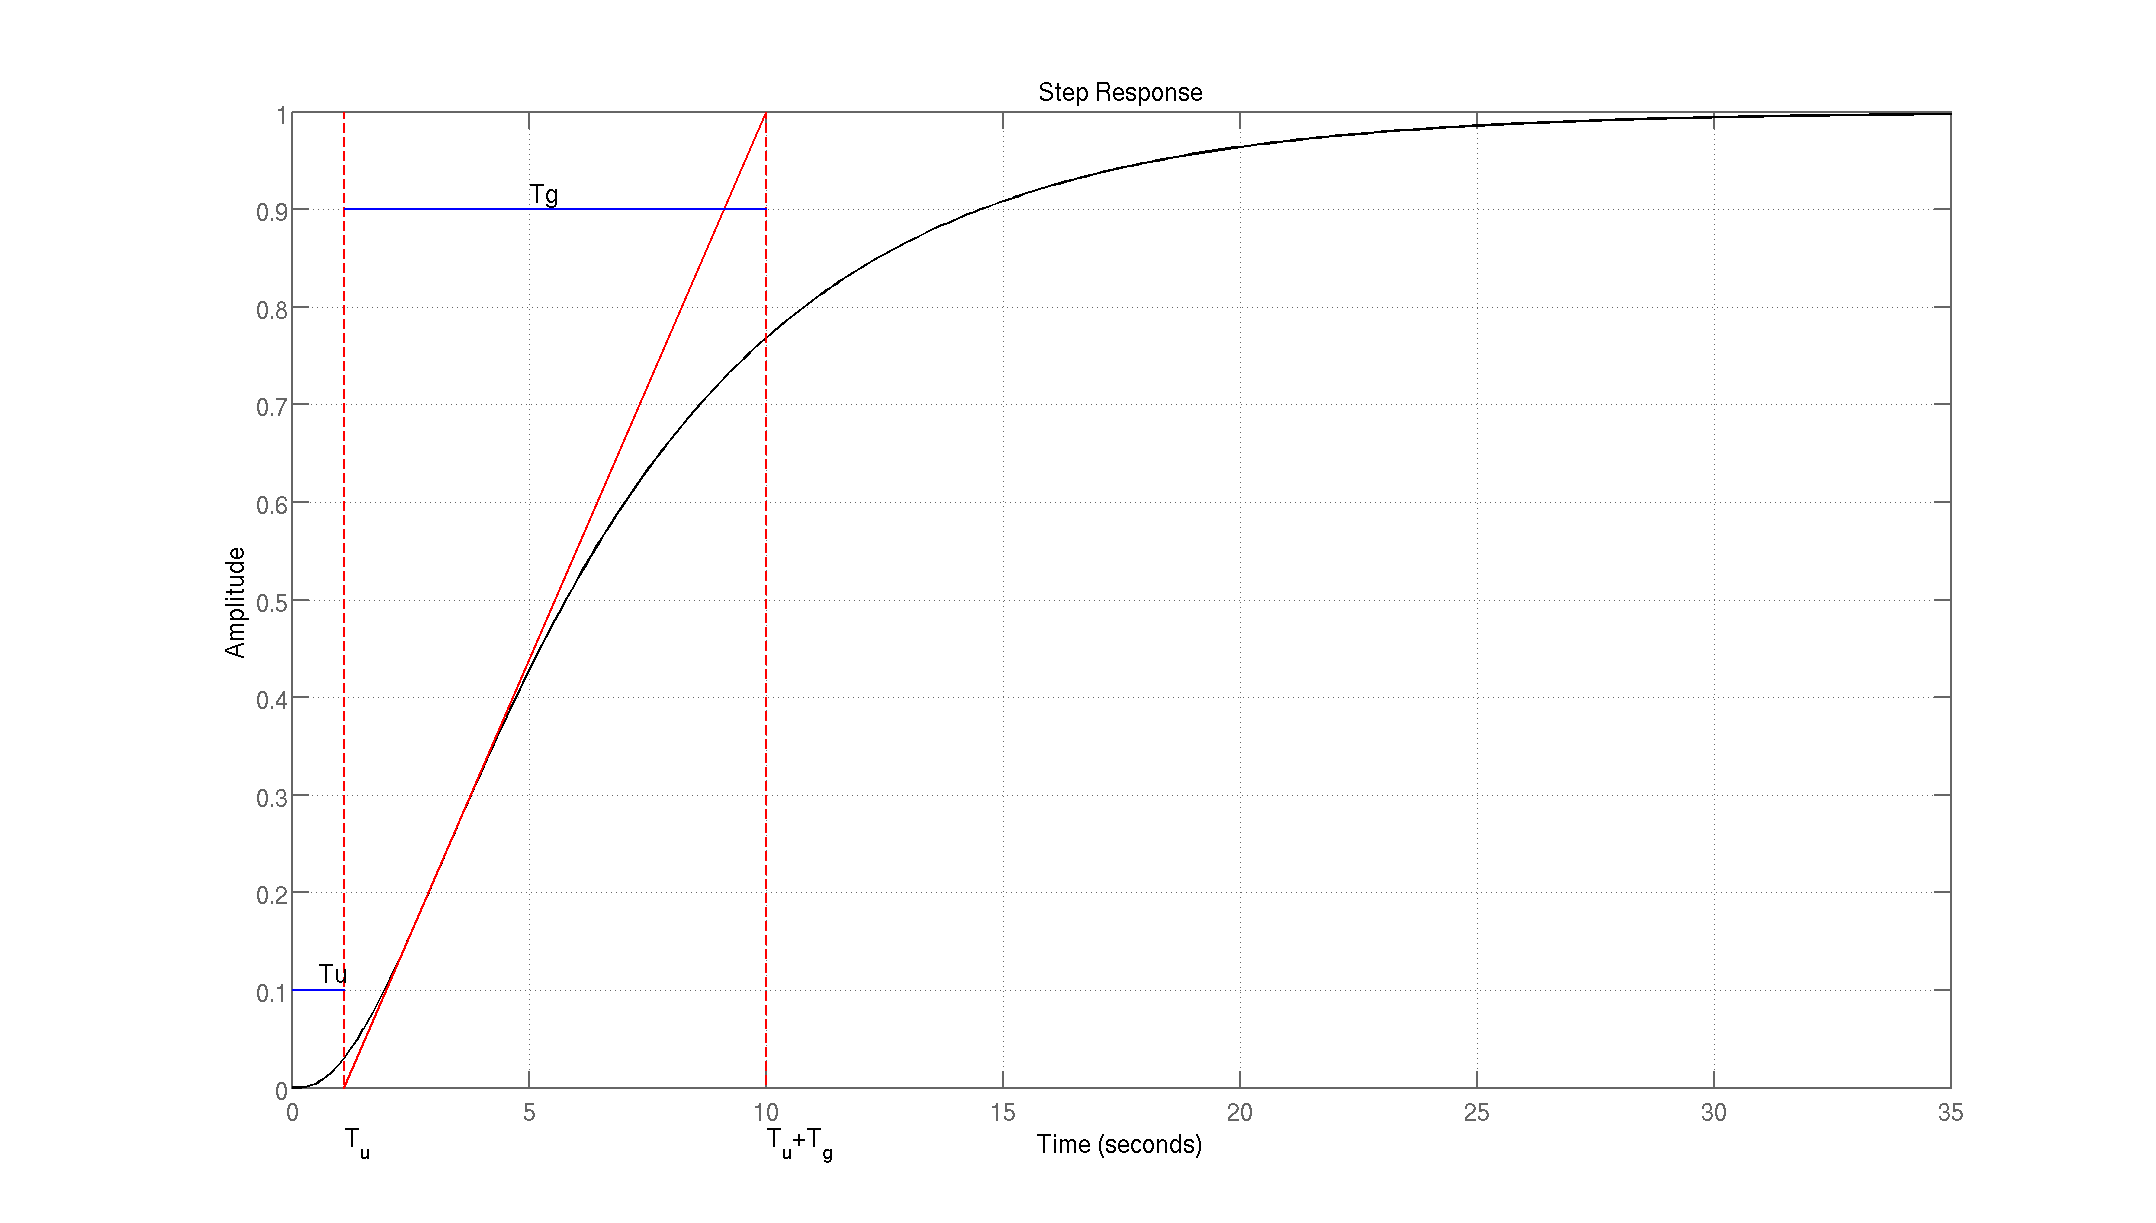
\includegraphics[width=.9\textwidth]{images/streckeSchrittantwort.png}
    \caption{%
    Schrittantwort der  Beispielstrecke (schwarz), Wendetangende  (rot), $T_u$
    und $T_g$ (blau)%
    }
    \label{fig:plant_step}
\end{figure}

Der  geschlossene   Regelkreis  soll  schlussendlich  maximal   etwa  $16.3\%$
\"uberschwingen.

Wir erhalten:
\begin{itemize}
    \item
        $K_s = \SI{2}{\second}$
    \item
        $T_u = \SI{1.1}{\second}$
    \item
        $T_g = \SI{8.9}{\second}$
\end{itemize}

Da  die Phasengangmethode  vom {\em{Frequenzgang}}  einer Strecke  ausgeht und
nicht von der Schrittantwort, besteht der n\"achste Schritt nun darin, aus den
obigen Werten  den Frequenzgang  der Strecke  zu bestimmen. Dies  erledigt die
methode \code{p\_sani}, welche uns  die Werte f\"ur die \"Ubertragungsfunktion
der  Strecke   liefert.  \todo{Allenfalls   Verweis  auf   Softwareteil  f\"ur
Erkl\"arungen  zu  sani-Methode.}   In  unserem  Fall  ergibt  dies  folgendes
Polynom:

\begin{gather} \label{eq:transfer:plant}
    \begin{split}
        H_s (s) & = K_s
                  \cdot \frac{1}{1 + s \cdot T_1}
                  \cdot \frac{1}{1 + s \cdot T_2}
                  \cdot \frac{1}{1 + s \cdot T_2}                     \\
                & = 2
                  \cdot \frac{1}{1 + s \cdot \SI{0.4134}{\second}}
                  \cdot \frac{1}{1 + s \cdot \SI{1.4894}{\second}}
                  \cdot \frac{1}{1 + s \cdot \SI{5.3655}{\second}}
    \end{split}
\end{gather}

Mit einem  geeigneten Tool  kann man sich  den dazugeh\"origen  Plot erstellen
lassen.

\begin{figure}[h! width=\pagewidth]
    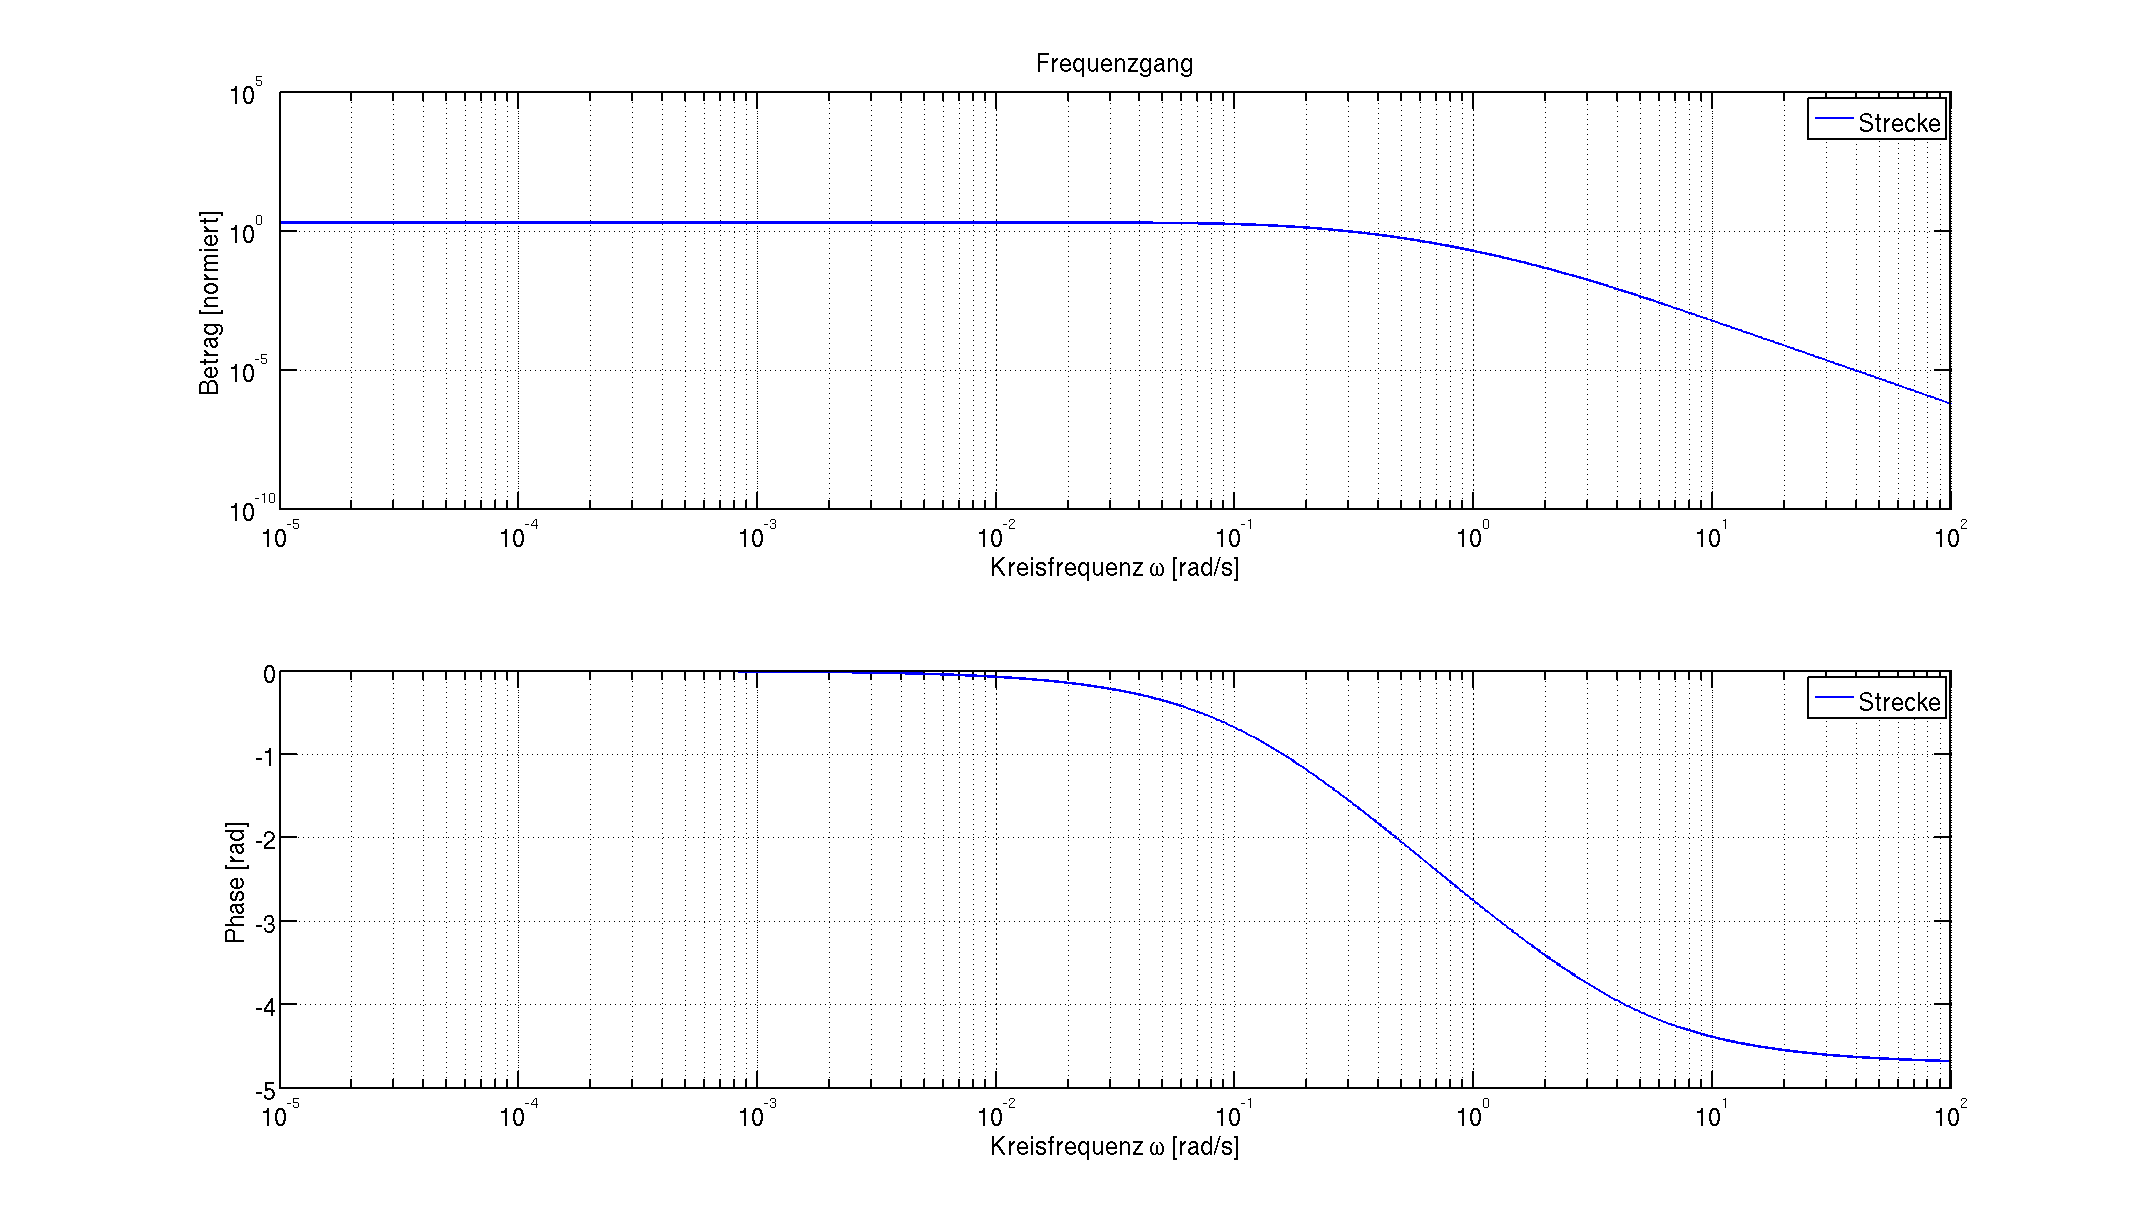
\includegraphics[width=.9\textwidth]{images/streckeFrequenzgang.png}
    \caption{%
        Frequenzgang der Strecke%
    }
    \label{fig:plant_freq}
\end{figure}

An diesem Punkt divergieren die Verfahren f\"ur den PI- und den PID-Regler. Es
soll zuerst der PI-Regler dimensioniert werden.

\subsubsection*{PI-Regler}

Das schlussendliche Ziel ist die Bestimmung der Parameter $K_{rk}$ und $T_{nk}$
in der Gleichung:

\begin{equation} \label{eq:pi:target}
    H_{rpi} = K_{rk} \cdot \biggl[ 1 + \frac{1}{s \cdot T_{nk}} \biggr]
\end{equation}

Zuerst wird im Phasengang der Strecke die Frequenz $\omega_{pi}$ bestimmt, f\"ur
welche die Phase der Strecke $-90\degree$ betr\"agt.

\begin{equation} \label{eq:pi:phi_s}
    \varphi_s(\omega_{pi}) = -90 \degree
\end{equation}

\begin{figure}[h! width=\pagewidth]
    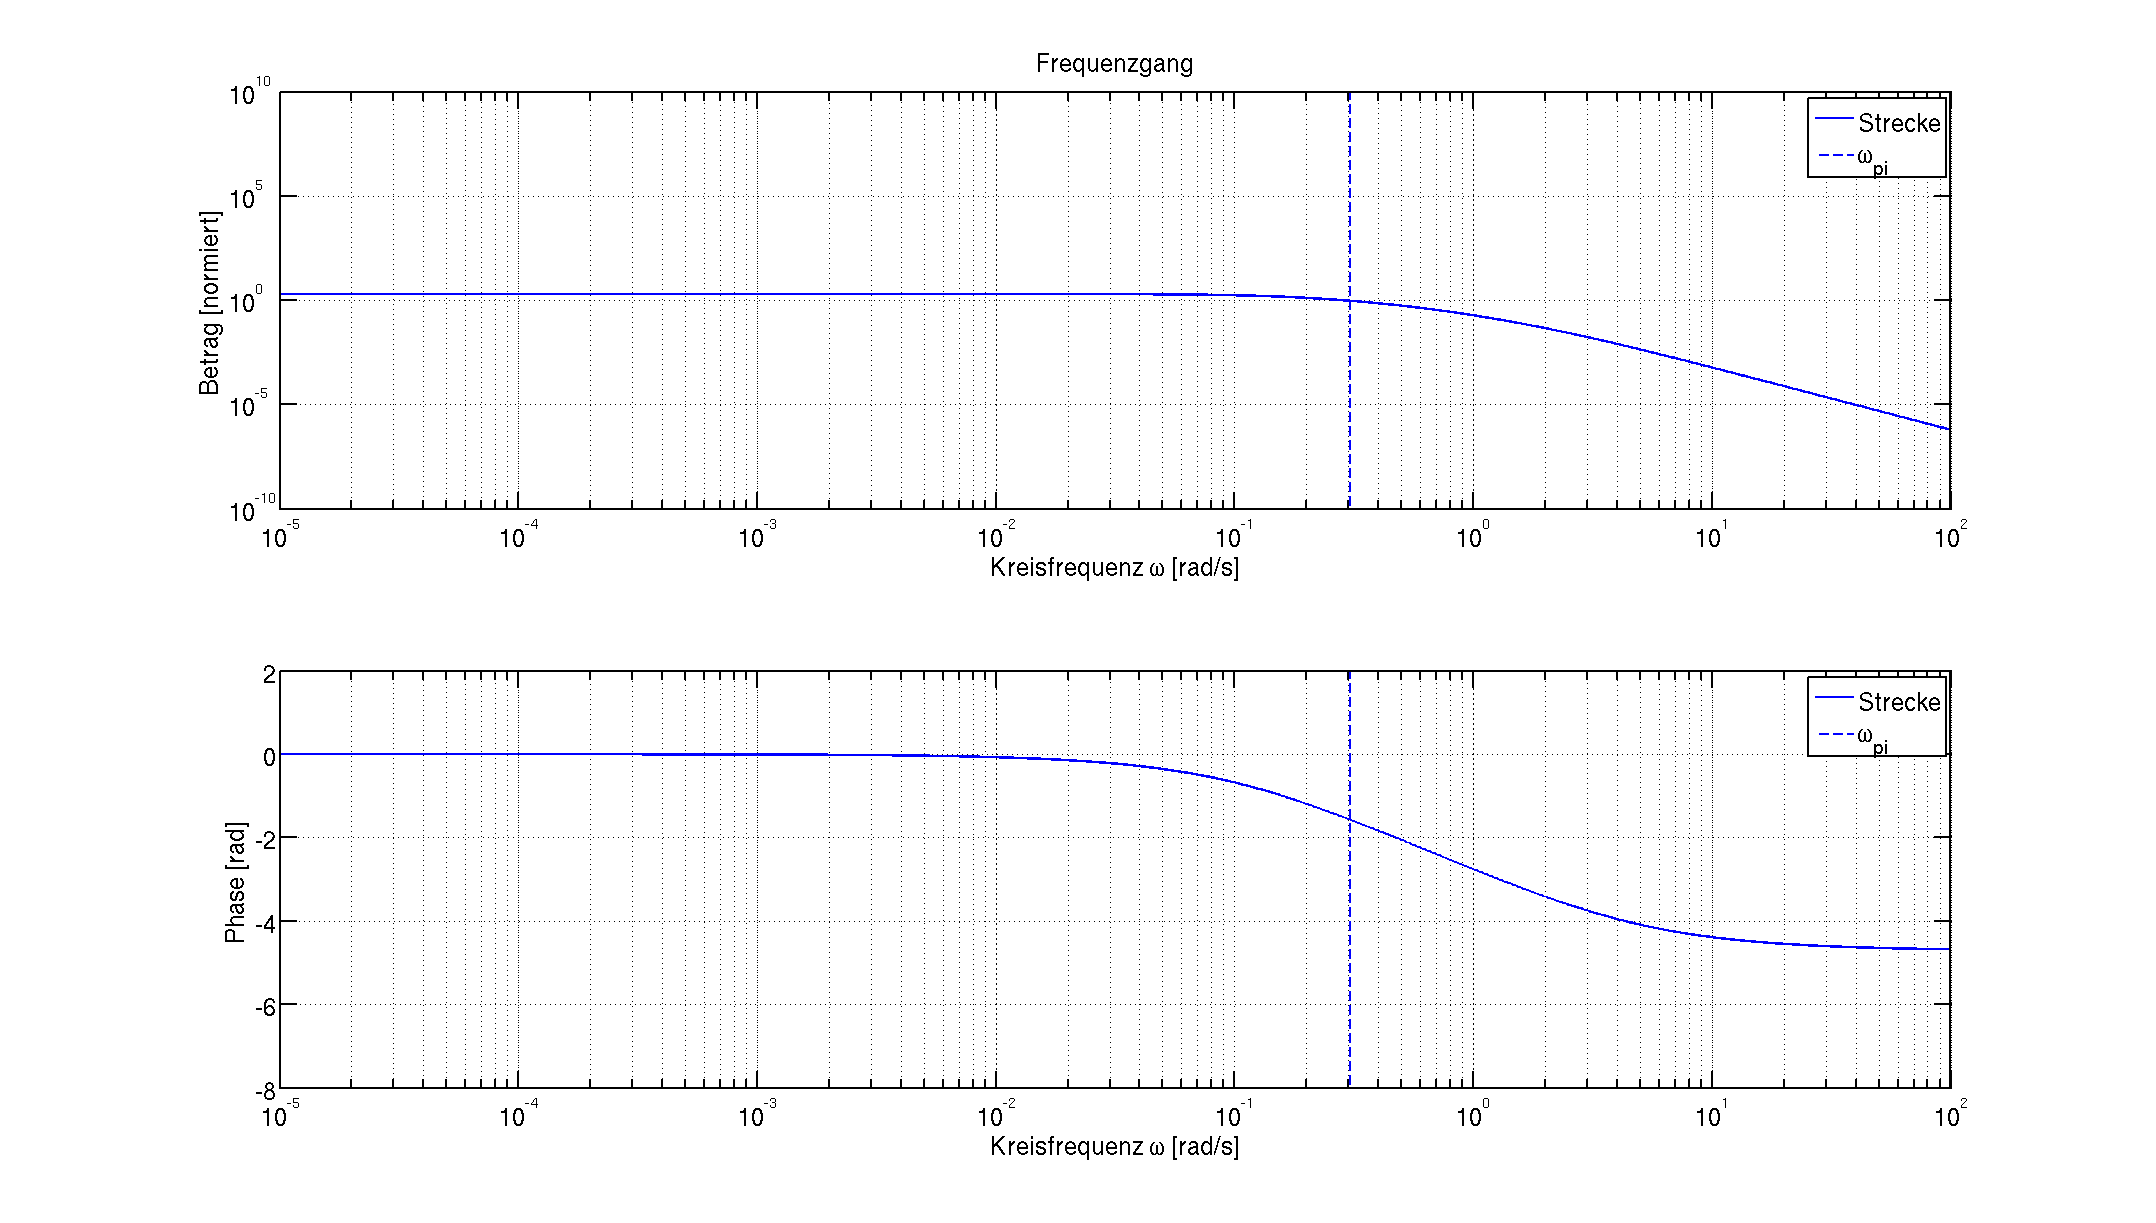
\includegraphics[width=.9\textwidth]{images/piStreckeOmegaPI.png}
    \caption{%
        $\omega_{pi}$ eingetragen (vertikale gestrichelte Linie).
    }
    \label{fig:pi:omega_pi}
\end{figure}

Wie man aus Abbildung \ref{fig:pi:phi_s} ablesen kann, liegt dieser Wert f\"ur
$\omega_{pi}$ in unserem  Beispiel bei ungef\"ahr $\SI{0.3}{\per\second}$. Die
Kontrollrechnung mittels Matlab ergibt:

\begin{equation} \label{eq:pi:omega_pi}
    \omega_{pi} = \SI{0.3039}{\per\second}
\end{equation}

Damit kann nun $T_{nk}$ direkt bestimmt werden\footnotemark[1]:

\begin{equation} \label{eq:pi:omega_pi}
    T_{nk} = \frac{1}{\omega_{pi}} = \frac{1}{\SI{0.3039}{\per\second}} = \SI{3.2902}{\second}
\end{equation}

\footnotetext[1]{
    Um die  Akkumulation von Ungenauigkeiten  zu minimieren werden  bei diesen
    Berechnungen  die  genauen  Werte  aus  Matlab  verwendet  und  nicht  die
    gerundeten  Zwischenresultate,  was  zu   Abweichungen  zu  den  von  Hand
    berechneten Ergebnissen f\"uhren kann.
}
\todo{Fragen ob dies OK ist.}

Als N\"achstes  soll die Durchtrittsfrequenz $\omega_d$  bestimmt werden. Dazu
wird  der  f\"ur  $T_{nk}$  erhaltene  Wert  in  Gleichung  \ref{eq:pi:target}
eingesetzt. Da $K_{rk}$ noch unbekannt ist, wird vorerst $K_{rk} = 1$ gesetzt.

\begin{gather} \label{eq:pi:target}
    \begin{split}
        H_{rpi} & = K_{rk} \cdot \biggl[ 1 + \frac{1}{s \cdot T_{nk}} \biggr] \\
                & = 1      \cdot \biggl[ 1 + \frac{1}{s \cdot \SI{3.2902}{\second}} \biggr]
    \end{split}
\end{gather}

Daraus   kann   nun   der   Frequenzgang   des   {\em{offenen   Regelkreises}}
(\"Ubertragungsfunktion $H_o$,  Amplitudengang $A_o$,  Phasengang $\varphi_o$)
bestimmt werden.

\begin{gather} \label{eq:pi:h_open}
    \begin{split}
        H_o (s) & = H_{rpi} (s) \cdot H_s (s) \\
            & = \Biggl(
                    K_{rk} \cdot \biggl[ 1 + \frac{1}{s \cdot T_{nk}} \biggr]
                \Biggr)
                \cdot
                K_s
                \cdot
                \Biggl(
                        \frac{1}{1 + s \cdot T_1}
                  \cdot \frac{1}{1 + s \cdot T_2}
                  \cdot \frac{1}{1 + s \cdot T_2}
                \Biggr) \\
            & = \Biggl(
                    1 \cdot \biggl[ 1 + \frac{1}{s \cdot \SI{3.2902}{\second}} \biggr]
                \Biggr)
                \cdot
                2
                \cdot
                \Biggl(
                          \frac{1}{1 + s \cdot \SI{0.4134}{\second}}
                    \cdot \frac{1}{1 + s \cdot \SI{1.4894}{\second}}
                    \cdot \frac{1}{1 + s \cdot \SI{5.3655}{\second}}
                \Biggr)
    \end{split}
\end{gather}


Wobei der Amplitudengang den Betragsverlauf und der Phasengang den Verlauf des
Arguments dieser \"Ubertragungsfunktion repr\"asentieren:
\todo{Allenfalls auch wirklich ausrechnen... w\"urde aber ziemlich langwierig.}

\begin{equation}
    \begin{split} \label{eq:pi:a_o_phi_o}
        A_o(j\omega)       & = |H_o(j\omega)| \\
        \varphi_o(j\omega) & = arg(H_o(j\omega))
    \end{split}
\end{equation}

Von besonderem  Interesse ist  hier der Phasengang. Wie  Anfangs spezifiziert,
soll  ein maximals  \"Uberschwingen von  ca. $16.3\%$ angestrebt  werden. Dazu
muss die Durchtrittsfrequenz $\omega_d$ gefunden werden, an welcher der offene
Regelkreis eine Phase von $-128.5\degree$ aufweist. \footnotemark[2]

\footnotetext[2]{%
    Wird ein anderes \"Uberschwingverhalten gew\"unscht, muss hier ein anderer
    Wert f\"ur die Durchtrittsfrequenz  $\omega_d$ bestimmt werden, siehe dazu
    Tabelle \ref{tab:phi_s}.
}

\begin{figure}[h! width=\pagewidth]
    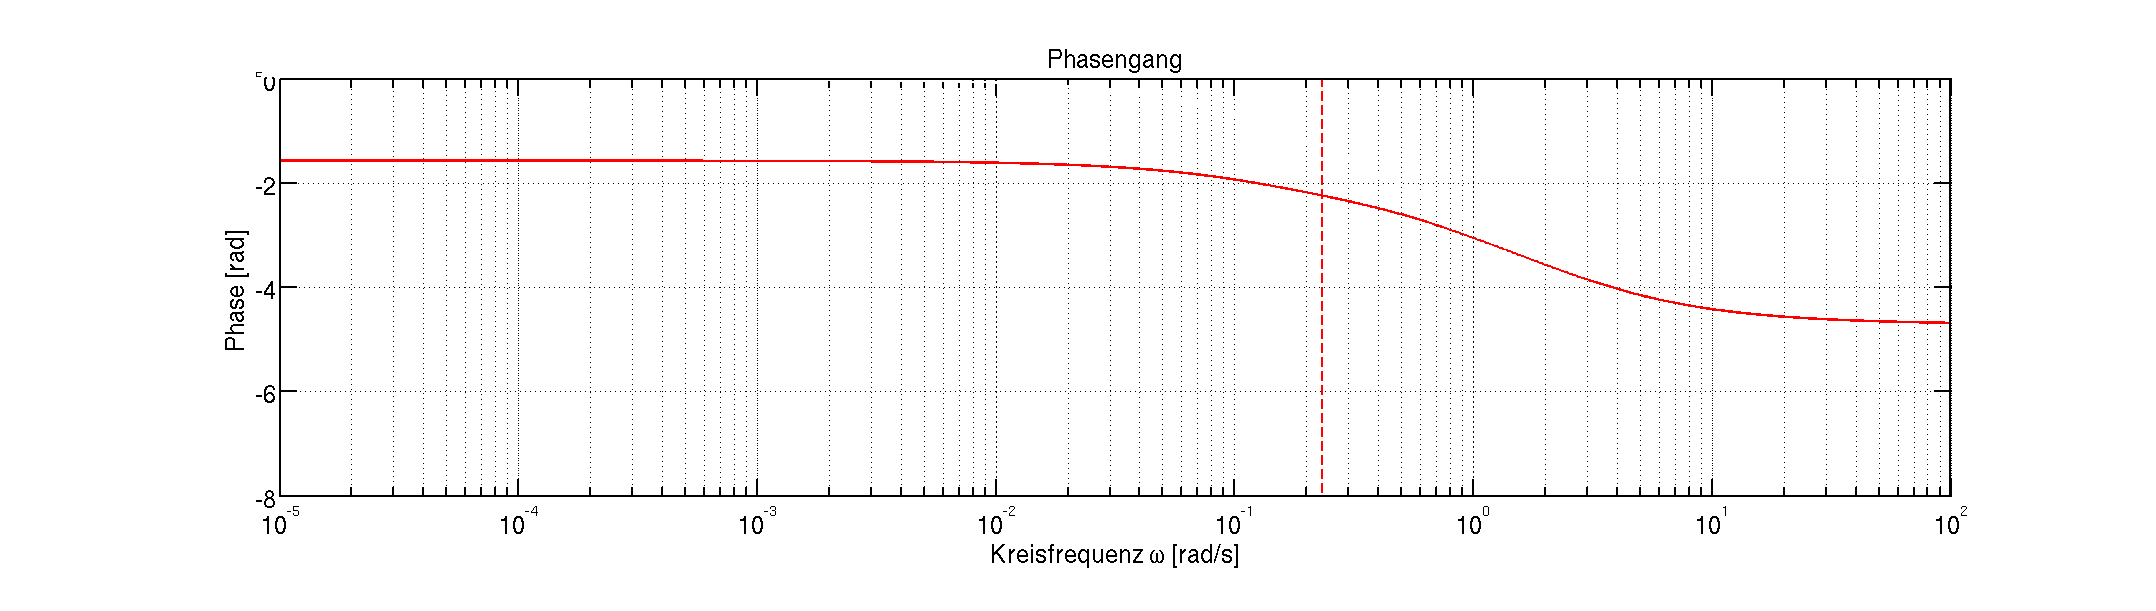
\includegraphics[width=.9\textwidth]{images/piOffenerRegelkreisPhasengang.png}
    \caption{%
        Phasengang   $\varphi_o(j\omega)$   des   offenen   Regelkreises   mit
        eingetragener Durchtrittsfrequenz $\omega_{d}$ (vertikale gestrichelte
        Linie). Wie man verifizieren kann, weist der offene Regelkreis unseres
        Beispiels bei dieser Kreisfrequenz  eine Phase von $-128.5\degree$ auf
        (etwa $\SI{-2.24}{\radian}$).
    }
    \label{fig:pi:omega_d}
\end{figure}

Dies ergibt:
\begin{equation} \label{eq:pi:omega_d}
    \omega_d = \SI{0.2329}{\per\second}
\end{equation}

In  einem  letzten  Schritt  wird  nun  die  Durchtrittsfrequenz  benutzt,  um
die  ben\"otigte Verst\"arkung  $K_{rk}$ des  Reglers zu  bestimmen. Dazu wird
$\omega_d$ in  Gleichung \ref{eq:pi:h_open}  eingesetzt, $|H_o(j\omega)|  = 1$
gesetzt    (Durchtrittsfrequenz: Frequenz,     bei    der     die    Amplitude
$\SI{0}{\decibel} = 1$ ist).

\begin{gather} \label{eq:pi:A_o_set_to_one}
    \begin{split}
        A_o & = | H_o (j\omega_d) | \\
            & = \abs*{
                    \bigg(
                        K_{rk} \cdot \biggl[ 1 + \frac{1}{j \cdot \omega_d \cdot T_{nk}} \biggr]
                    \bigg)
                    \cdot
                    K_s
                    \cdot
                    \bigg(
                            \frac{1}{1 + j \cdot \omega_d \cdot T_1}
                      \cdot \frac{1}{1 + j \cdot \omega_d \cdot T_2}
                      \cdot \frac{1}{1 + j \cdot \omega_d \cdot T_2}
                      \bigg)} \\
              & = 1
    \end{split}
\end{gather}

Mit den Werten
\begin{equation} \label{eq:pi:values}
    \begin{split}
        K_s      & = 2                    \\
        T_{nk}   & = \SI{3.2902}{\second} \\
        T_1      & = \SI{0.4134}{\second} \\
        T_2      & = \SI{1.4894}{\second} \\
        T_3      & = \SI{5.3655}{\second} \\
        \omega_d & = \SI{0.2329}{\radian\per\second}
    \end{split}
\end{equation}

l\"ost  man Gleichung  \ref{eq:pi:A_o_set_to_one}  nun nach  $K_{rk}$ auf  und
erh\"alt:

\begin{equation} \label{eq:pi:k_rk_result}
    K_{rk} = 0.517577
\end{equation}

Somit ist der PI-Regler vollst\"andig bestimmt und hat folgende Form:

\begin{equation} \label{eq:pi:result}
    H_{rpi} = 0.518 \cdot \biggl[ 1 + \frac{1}{s \cdot \SI{3.29}{\second}} \biggr]
\end{equation}

Zum Vergleich das Bode-Diagramm mit allen relevanten Kurven und Werten:
\begin{figure}[h! width=\pagewidth]
    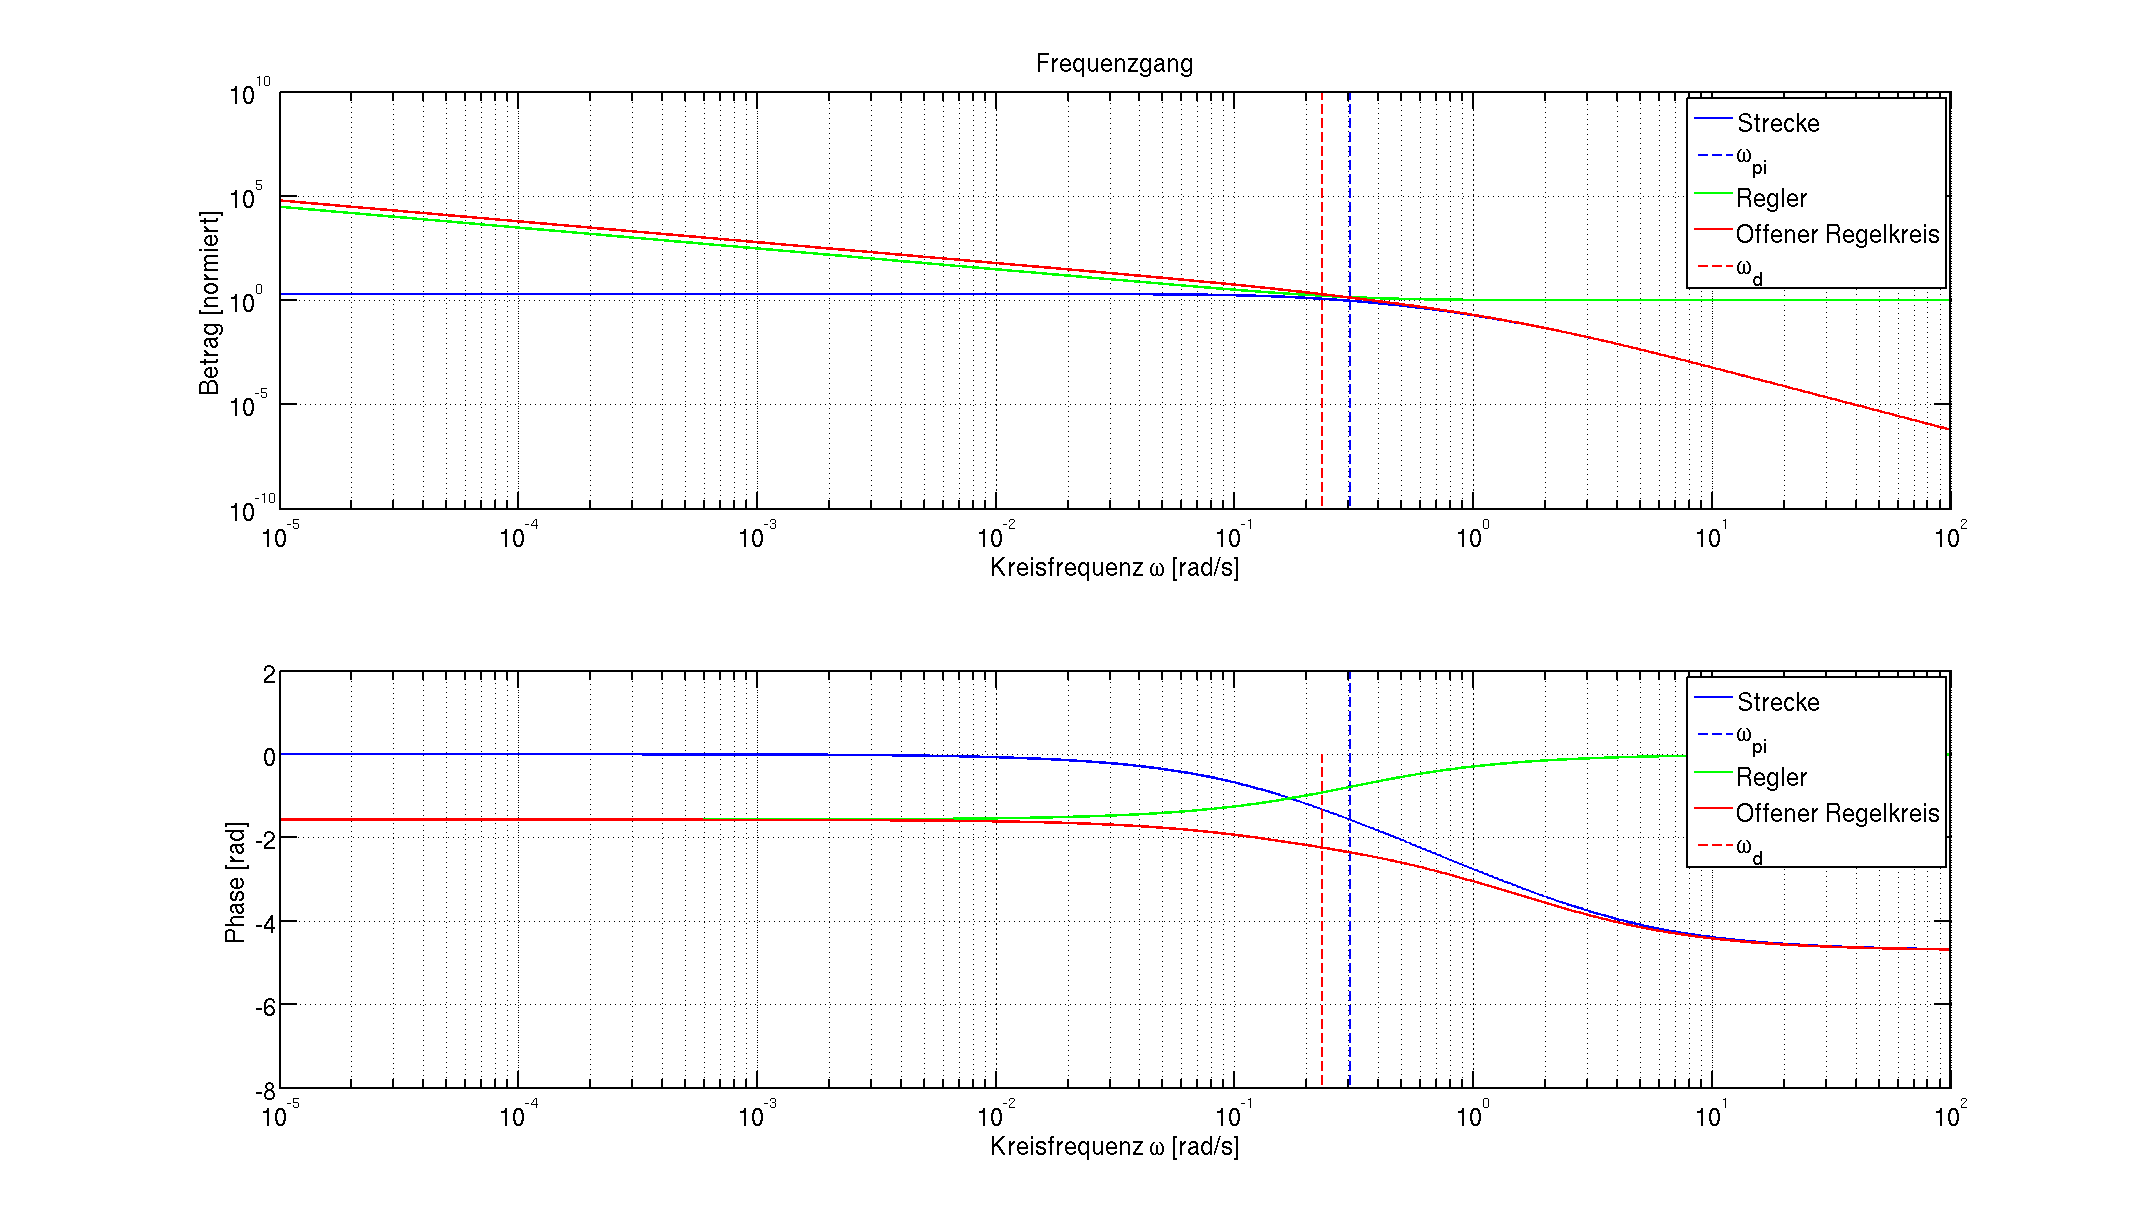
\includegraphics[width=.9\textwidth]{images/piBode.png}
    \caption{%
        Frequenzgang des Reglers (gr\"un), der  Strecke (blau) und des offenen
        Regelkreises (rot).
    }
    \label{fig:pi:all}
\end{figure}
\todo{Fix vertical line $\omega_d$}



\subsubsection*{PID-Regler}

Das schlussendliche Ziel ist die Bestimmung der Parameter $K_{rk}$, $T_{nk}$ und $T_{vk}$
in der Gleichung:

\begin{equation} \label{eq:pid:target}
    H_{rpid} = K_{rk} \cdot \biggl[ \frac{(1 + s \cdot T_{nk}) \cdot (1 + s \cdot T_{vk}) }{ s \cdot T_{nk} } \biggr]
\end{equation}

Analog  zum PID-Regler  wird zuerst  im  Phasengang der  Strecke die  Frequenz
$\omega_{pid}$  bestimmt, f\"ur  welche  die Phase  der Strecke  $-135\degree$
betr\"agt.

\begin{equation} \label{eq:pid:phi_s}
    \varphi_s(\omega_{pid}) = -135 \degree
\end{equation}

In unserem Beispiel ergibt dies:

\begin{equation} \label{eq:pid:omega_pid}
    \omega_{pid} = \SI{0.6714}{\per\second}
\end{equation}

Anschliessend wird die  Steigung des Phasengangs $\varphi_s$  bei der Frequenz
$\omega_{pid}$ bestimmt, ausgehend von der \"Ubertragungsfunktion der Strecke,
welche \code{p\_sani} berechnet hat (siehe Gleichung \ref{eq:transfer:plant}).

\begin{equation} \label{eq:transfer:plant:derivative}
    \frac{d\varphi_s}{d\omega} \biggr \rvert_{\omega=\omega_{pid}}
        = \frac{d(arg(H_s(j\omega)))}{d\omega} \biggr \rvert_{\omega=\omega_{pid}}
        = \SI{-1.5124}{\second}
\end{equation}
\todo{Einheit \"uberpr\"ufen}

Zwischen den Steigungen der Phasen des offenen Regelkreises ($\varphi_o$), der
Strecke ($\varphi_s$) und des Reglers ($\varphi_r$) gilt folgende Beziehung:

\begin{equation} \label{eq:pid:phi_sum}
    \varphi_o = \varphi_s + \varphi_r
\end{equation}
\todo{Verweis auf plot}

Es soll nun gelten:

\begin{equation} \label{eq:pid:dphi_o_target}
    \frac{\varphi_o}{d\omega} \biggr \rvert_{\omega=\omega_{pid}} = - \frac{1}{2}
\end{equation}

Es ist also  ein passender Wert f\"ur $\varphi_r$  gesucht, sodass Gleichungen
\ref{eq:pid:phi_sum}  und  \ref{eq:pid:dphi_o_target}   erf\"ullt  sind  unter
Ber\"ucksichtigung des Resultats von \ref{eq:transfer:plant:derivative}.

Dazu f\"uhrt man den Hilfsparameter $\beta$ ein, f\"ur den gilt:


\begin{gather} \label{eq:pid:beta:start}
    \begin{split}
        \frac{1}{T_{vk}} & = \frac{\omega_{pid}}{\beta} \\
        \frac{1}{T_{nk}} & = \omega_{pid} \cdot \beta  \\
                       0 & <  \beta \leq 1
    \end{split}
\end{gather}

Die  beiden Frequenzen  $\frac{1}{T_{vk}}$  und  $\frac{1}{T_{nk}}$ sind  also
symmetrisch  um den  Faktor $\beta$  gr\"osser bzw.  kleiner als  die Frequenz
$\omega_{pid}$. \todo{siehe Plot} Will man  $\beta$ von Hand bestimmen, trifft
man zuerst eine ``vern\"unftige'' Annahme, zum Beispiel:

\begin{equation} \label{eq:pid:beta:initial_value}
    \beta = 0.5
\end{equation}

Mit  diesem Startwert  bestimmt  man nun  $T_{nk}$  und ${T_{vk}}$. Die  somit
erhaltenen Werte setzt man in  Gleichung \ref{eq:pid:target} ein, zusammen mit
dem Wert f\"ur $\omega_{pid}$ aus Gleichung \ref{eq:pid:omega_pid}:

\begin{gather} \label{eq:pid:t_nk_t_vk_initial_results}
    \begin{split}
        {T_{vk}} & = \frac{\beta}{\omega_{pid}}  = \frac{0.5}{\SI{0.6714}{\per\second}}                   = \SI{0.7447}{\second} \\
        {T_{nk}} & = \frac{1}{\omega_{pid} \cdot \beta} = \frac{1}{\SI{0.6714}{\per\second} \cdot 0.5 }  = \SI{2.9789}{\second} \\
    \end{split}
\end{gather}

Eingesetzt in die Reglergleichung, vorerst mit $K_{rk} = 1$:

\begin{gather} \label{eq:pid:t_nk_t_vk_initial_results}
    \begin{split}
        H_{rpid} & = K_{rk} \cdot \biggl[ \frac{(1 + j\omega \cdot T_{nk}) \cdot (1 + j\omega \cdot T_{vk}) }{ j\omega \cdot T_{nk} } \biggr] \\
                 & = 1      \cdot \biggl[ \frac{(1 + j\omega \cdot \SI{2.9789}{\second}) \cdot (1 + j\omega \cdot \SI{0.7447}{\second}) }{ j\omega \cdot  \SI{2.9789}{\second}} \biggr]
    \end{split}
\end{gather}

Von dieser Gleichung bestimmt man nun den Phasengang und wertet danach dessen
Ableitung an der Stelle $\omega = \omega_{pid}$ aus:

\begin{gather} \label{eq:pid:phi_r_first_iteration}
    \begin{split}
        \varphi_s (j\omega)                                            & = arg(H_{rpid}(j\omega))        \\
        \frac{d\varphi_s}{d\omega} \biggr \rvert_{\omega=\omega_{pid}} & = \SI{1.1920}{\second}
    \end{split}
\end{gather}
\todo{Die zugeh\"orige Rechnung ist lange und m\"uhsam, allenfalls in Anhang? Ebenfalls: Einheit kontrollieren}


Setzt man dies in Gleichung \ref{eq:pid:phi_sum} ein, erh\"alt man:
\begin{equation} \label{eq:pid:phi_sum_result_iteration_one}
    \varphi_o = \varphi_s + \varphi_r =\SI{-1.5124}{\second} + \SI{1.1920}{\second} = \SI{-0.3204}{\second} > -\frac{1}{2}
\end{equation}

Mit  $\beta  = 0.5$  erh\"alt  man  also eine  zu  hohe  Steigung des  offenen
Regelkreises   and   der   Stelle  $\omega_{pid}$,   folglich   muss   $\beta$
{\em{verkleinert}} werden.   Diese Berechnungen  werden nun mit  jeweils neuen
Werten  f\"ur  $\beta$  solange  wiederholt,  bis  die  Steigung  des  offenen
Regelkreises die gew\"unschte N\"ahe zu $-\frac{1}{2}$ aufweist.

Da die manuelle Iterierung dieses Prozesses enorm viel Zeit in Anspruch nimmt,
bietet  sich  hier  eine  Automatisierung  an. Die  Berechnung  mittels  eines
geeigneten Algorithmus in Matlab liefert schlussendlich folgendes Ergebnis:
\todo{Allenfalls Matlab-Algo in Anhang und Verweis}

\begin{gather} \label{eq:pid:beta_result}
    \begin{split}
        \beta    & = 0.2776 \\
        {T_{vk}} & = \frac{\beta}{\omega_{pid}}           = \SI{0.4134}{\second} \\
        {T_{nk}} & = \frac{1}{\omega_{pid} \cdot \beta}   = \SI{5.3656}{\second} \\
    \end{split}
\end{gather}

Sollte  man  f\"ur  $\beta$  einen komplexen  Wert  erhalten,  wird  $\beta=1$
gesetzt.\todo{Wie kann dies egtl. passieren?}

Dieser Werte setzt man nun in Gleichung \ref{eq:pid:target} ein. $K_{rk}$ wird
wie bei der Bestimmung von $\beta$ vorerst noch auf 1 gesetzt.

\begin{gather} \label{eq:pid:h_rpid_beta_result}
    \begin{split}
        H_{rpid} & = K_{rk} \cdot \biggl[ \frac{(1 + s \cdot T_{nk}               ) \cdot (1 + s \cdot T_{vk}               ) }{ s \cdot T_{nk}               } \biggr]
                   = 1      \cdot \biggl[ \frac{(1 + s \cdot \SI{5.3656}{\second} ) \cdot (1 + s \cdot \SI{0.4134}{\second} ) }{ s \cdot \SI{5.3656}{\second} } \biggr]
    \end{split}
\end{gather}

Zur  Bestimmung   von  $K_{rk}$   wird  nun   der  Frequenzgang   des  offenen
Regelkreises    betrachtet. Dazu   multipliziert    man    wie   gehabt    die
\"Ubertragungsfunktion der  Strecke (siehe  Gleichung \ref{eq:transfer:plant})
mit  der  soeben  bestimmten  \"Ubertragungsfunktion  des  Reglers  (Gleichung
\ref{eq:pid:h_rpid_beta_result}).

\begin{equation} \label{eq:pid:h_o_k_rk_one}
    H_{o}(j\omega) = H_{rpid}(j\omega) \cdot H_s(j\omega)
\end{equation}

Nun wird  die Durchtrittsfrequenz $\omega_d$  bestimmt, an welcher  der offene
Regelkreis eine  Verst\"arkung von $\SI{0}{\decibel} =  1$ aufweisen soll. Wie
auch  beim  PI-Regler  werden  wir   hier  ein  \"Uberschwingen  von  $16.3\%$
anstreben, womit gilt:

\begin{equation} \label{eq:pid:omega_d_target}
    \varphi_s(\omega_d) = \varphi_s = -128.5\degree
\end{equation}

Dieser Wert wird analog zum PI-Regler aus dem Phasengang des offenen Regelkreises
abgelesen. \todo{siehe Plot} Eine Berechnung mittels Matlab ergibt:


\begin{equation} \label{eq:pid:omega_d_target}
    \omega_d = \SI{0.5341}{\per\second}
\end{equation}

In einem letzten Schritt wird  nun der Amplitudengang des offenen Regelkreises
an der  Stelle $\omega_d$ gleich 1  gesetzt und diese Gleichung  nach $K_{rk}$
aufgel\"ost:

\begin{equation} \label{eq:pid:h_o_k_rk_one}
    \begin{split}
        A_{o}(j\omega_d)    & = | H_{o}(j\omega_d) |                            \\
                            & = | H_{rpid}(j\omega_d) \cdot H_s(j\omega_d) |    \\
                            & = \Biggl \rvert
                                    K_{rk}
                                    \cdot
                                    \biggl[ \frac{(1 + j\omega_d \cdot T_{nk}) \cdot (1 + j\omega_d \cdot T_{vk}) }{ j\omega_d \cdot T_{nk} } \biggr] \Biggr \rvert \\
                            & \cdot
                                \Biggl \rvert
                                    K_s
                                    \cdot \frac{1}{1 + j\omega_d \cdot T_1}
                                    \cdot \frac{1}{1 + j\omega_d \cdot T_2}
                                    \cdot \frac{1}{1 + j\omega_d \cdot T_2}
                                    \Biggr \rvert \\
                            & = 1
    \end{split}
\end{equation}

Mit den gegebenen und berechneten Werten:
\begin{gather} \label{eq:pid:h_o_k_rk_one}
    \begin{split}
        K_s         & = 2                        \\
        T_1         & = \SI{0.4134}{\second}     \\
        T_2         & = \SI{1.4894}{\second}     \\
        T_3         & = \SI{5.3655}{\second}     \\
        T_{nk}      & = \SI{5.3656}{\second}     \\
        T_{vk}      & = \SI{0.4134}{\second}     \\
        \omega_d    & = \SI{0.5341}{\per\second}
    \end{split}
\end{gather}

Dies liefert:

\begin{equation} \label{eq:pid:k_rk_result}
    K_{rk} = 1.83084
\end{equation}

Somit ist der Regler vollst\"andig bestimmt und hat folgende \"Ubertragungsfunktion:

\begin{equation} \label{eq:pid:target}
    H_{rpid}(s) = 1.83084 \cdot \biggl[ \frac{(1 + s \cdot \SI{5.3656}{\second} ) \cdot (1 + s \cdot \SI{0.4134}{\second} ) }{ s \cdot \SI{5.3656}{\second} } \biggr]
\end{equation}

Die Frequenzg\"ange der Strecke, des Reglers und des offenen Regelkreises:

\begin{figure}[h! width=\pagewidth]
    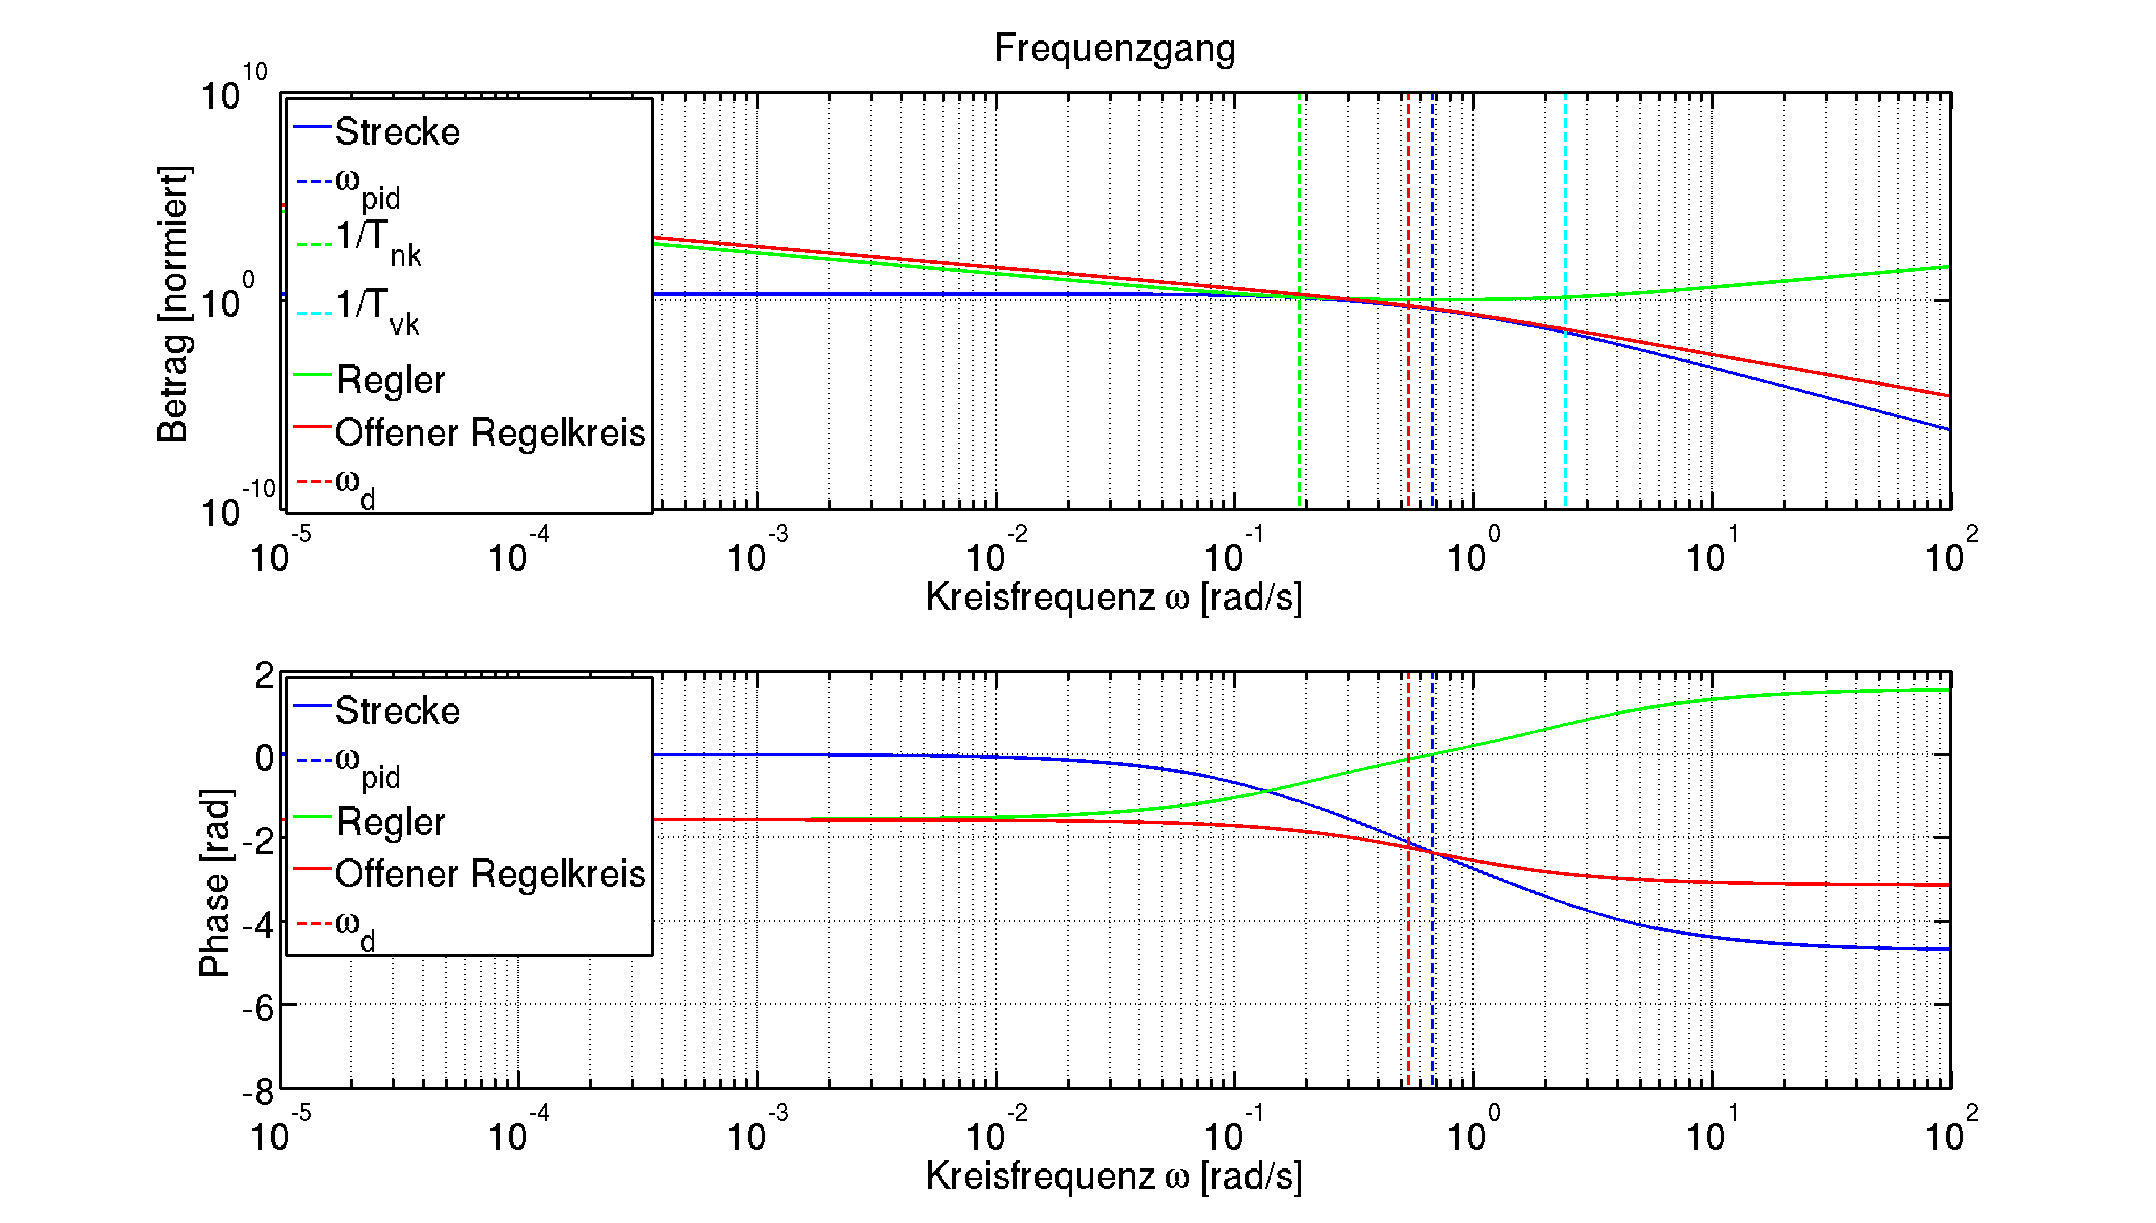
\includegraphics[width=.9\textwidth]{images/pidCompletePlot.png}
    \caption{%
        Frequenzgang der Strecke (blau), des  Reglers (gr\"un) und des offenen
        Regelkreises  (rot).  Ebenfalls  eingetragen  sind die  Reglerfrequenz
        $\omega_{pid}$,   die   beiden   Frequenzen   $\frac{1}{T_{vk}}$   und
        $\frac{1}{T_{nk}}$ sowie die Durchtrittsfrequenz $\omega_d$.
    }
    \label{fig:plant_step}
\end{figure}


\subsection{Schrittantwort des geschlossenen Regelkreises}
\todo{Abschnitt muss noch verfasst werden.}
Die    Aufgabe   eines    geschlossenen    Regelkreises (Abbildung \ref{fig:geschlossenerRegelkreis}) ist  es, einen  vorgegeben Sollwert  zu erreichen  und diesen
auch bei  St\"orungen aufrecht zu  erhalten. Dabei sollen die  unten genannten
dynamischen  Anforderungen  eingehalten  werden, damit  die  Stabilit\"at  des
Regelsystems garaniert ist. Die wichtigste  Bedingung f\"ur die Schrittantwort
ein  geschlossenen  Regelkreis heisst,  dass  der  Regelfehler, die  Differenz
zwischen Ist-und Sollwert, gleich Null oder m\"oglichst klein ist.\\


\begin{figure}[!h!, width=\pagewidth]
\begin{center}
    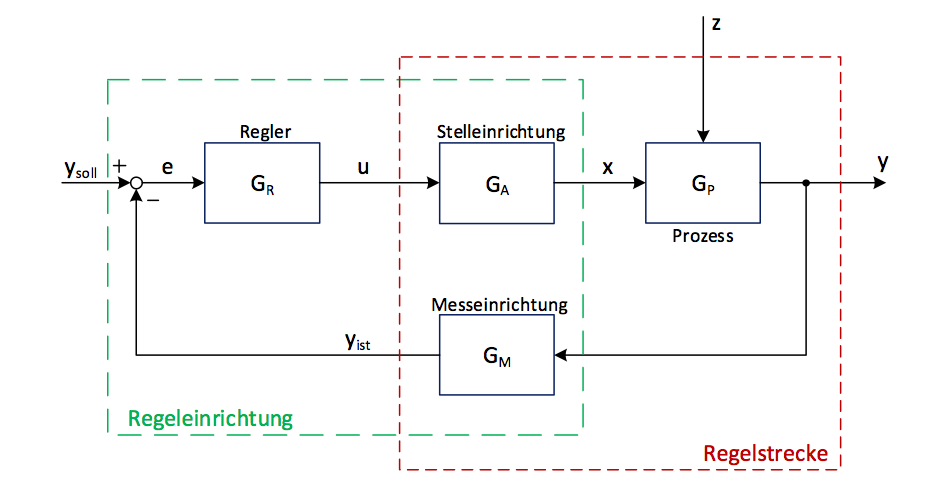
\includegraphics[width=0.5\textwidth]{images/geschlRegelkreis}
    \caption{Geschlossener Regelkreis}
    \label{fig:geschlossenerRegelkreis}
\end{center}
\end{figure}

%Name Bild Struktur eines allgemeinen Regelkreises
\begin{itemize}
    \item
        $y_soll$ bezeichnet den Sollwert der Regelgr\"osse.
    \item
        $e$ Regelabweichung (Regelfehler)
    \item
        $u$ Steuergr\"osse
    \item
        $x$ Stellgr\"osse
    \item
        $y$ Regelgr\"osse
    \item
        $z$ St\"orgr\"osse
    \item
        $y_ist$  ist der  Ist-Wert der  Regelgr\"osse  und wird  auch als  die
        Schrittantwort des Regelkreis bezeichnet.
\end{itemize}

\todo{Bild Schrittantworten passend zu Aufzählung unten}

Grunds\"atzlich  k\"onnen  f\"unf   Anforderungen  f\"ur  einen  geschlossenen
Regelkreis und deren Schrittantworten zusammengefasst werden:\\
\begin{enumerate}
    \item Der Regelkreis muss stabil sein:
        \begin{itemize}
            \item
                Das heisst  f\"ur die Schrittantwort, dass  nach dem Erreichen
                des  eingeschwungenen  Zustand kein  erneutes  \"Uberschwingen
                stattfinden darf.
            \item
                F\"ur  das  Regelsystem  heisst  stabil,  dass  es  in  seinen
                Gleichgewichtszustand zur\"uckgef\"uhrt werden kann.
        \end{itemize}
    \item
        Der Regelkreis  muss gen\"ugend ged\"ampft sein: \\Die  D\"ampfung der
        Schrittantwort soll  so stark  sein, dass der  eingeschwungene Zustand
        m\"oglichst  rasch erreicht  wird  ohne dass  das \"Uberschwingen  des
        Systems zu stark wird.
    \item
        Der   Regelkreis   muss   eine  bestimmte   station\"are   Genauigkeit
        aufweisen: Das  bedeutet,  der  Regelfehler  e(t) soll  f\"ur  t->  oo
        gegen  Null  gehen. F\"ur  die  Schrittantwort heisst  das,  dass  die
        Schrittantwort gleich $y_soll$ sein muss.
    \item
        Der Regelkreis  muss hinreichend  schnell sein: Die  Schnelligkeit des
        Einschwingvorganges der  Schrittantwort ist  stark von  der D\"ampfung
        abh\"angig. Ist die D\"ampfung  zu stark oder zu  schwach, braucht der
        Einschwingvorgang mehr Zeit. Hierbei muss darauf geachtet werden, dass
        die spezifischen Anforderungen an das Regelsystem eingehalten werden.
    \item
        Der  Regelkreis muss  robust  sein: Der Regelkreis  muss so  ausgelegt
        werden,  dass  das  Regelsystem  auch im  schlimmsten  Fall  (je  nach
        Regelsystem situationsabh\"angig) in der Lage ist, das System zur\"uck
        in den stabilen Zustand (vgl. 1.) zu regeln.
\end{enumerate}

